\begin{frame}{Embeddings}
    \begin{itemize}
        \item<1-> by embeddings we mean representing each textual feature as a dense vector in a low dimensional space
        \item<2-> how should we define these dense vectors or embeddings?
    \end{itemize}
\end{frame}
\begin{frame}{Word Embeddings}
    \begin{itemize}
        \item dense representations of words in an embedding space is known as word embeddings
        \item how to obtain word embeddings?  
    \end{itemize}
\end{frame}
\begin{frame}{Random Initizalization}
    \begin{itemize}
        \item<1-> we initialize the embedding vectors to random values
        \item<2-> values are uniformly sampled from numbers in the range
        \begin{itemize}
            \item<3->  $[-\frac{1}{2d}, +\frac{1}{2d} ] $ where $d$ is the number of dimensions (Mikolov et al., 2013)
            \item<4->  $[-\frac{\sqrt{6}}{\sqrt{d}}, +\frac{\sqrt{6}}{\sqrt{d}} ] $ (xavier initialization)
        \end{itemize}
    \end{itemize}
\end{frame}
\begin{frame}{Word Embeddings}
    \begin{itemize}
        \item<1-> dense representations of words in an embedding space is known as word embeddings
        \item<2-> these vectors can be obtained by random initialization and tuned for any NLP task
        \item<3-> however, we as human beings can define semantic relations between words independent of any NLP task
        \begin{itemize}
        \item e.g., ``blue'' and  'black'' are colors
        \item e.g., ``dog'' is more similar to ``cat'' than to ``chair'' 
        \item e.g., ``easy'' is the opposite of ``difficult''
        \end{itemize}
        \item<4-> how can we find word embeddings such that vectors of words with similar meaning be close to each other in the embedding space?
    \end{itemize}
\end{frame}
\begin{frame}{Word Meaning}
\begin{itemize}
    \item<1-> ``you should know a word by the company it keeps'' (Frith, 1957)
\end{itemize}
\begin{figure}
    \centering
    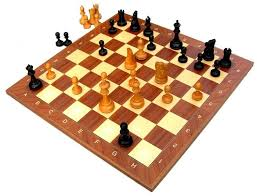
\includegraphics{./figure/chess.jpg}
\end{figure}
\end{frame}
\begin{frame}{Distributional Hypothesis}
\begin{itemize}
    \item<1-> words that occur in the same contexts tend to have similar meanings (Harris, 1945)
    \item<2-> how can we model the distributional hypothesis?
\end{itemize}
\end{frame}
\begin{frame}{Word-Context Matrix}
\begin{itemize}
    \item<1-> we count how often a word has occurred with a context in texts from a large corpus
    \item<2-> context is defined by a window over words
    \item<3-> let $V$ be the set of words in vocabulary and $C$ be the set of possible contexts
    \item<4-> word-context matrix $M$ is a two dimensional matrix whose rows are associated with $V$ and columns with $C$
    \item<5-> each entry of the matrix indicates how often a word co-occurs with a context in the given corpus
    \item<6-> this matrix is also known as co-occurrence matrix
\end{itemize}
\end{frame}
\begin{frame}{Word-Context Matrix}
\begin{itemize}
    \item corpus:
\begin{itemize}
    \item I like DL
    \item I like NLP
    \item I love ML
    \item I love NLP
\end{itemize}
\item window size = 1

\end{itemize}
\uncover<2->
{
\begin{table}[!h]
    \centering
    \begin{tabular}{l|cccccc}
          &  I & like & love & DL & NLP &ML  \\
          \hline
         I & 0 & 2 & 2 & 0 &0 &0  \\
         like & 2 & 0 & 0 & 1 & 1 &0 \\
         love & 2 & 0 & 0 & 0 & 1 & 1 \\
         DL & 0 & 1 & 0 & 0 & 0 & 0 \\
         NLP & 0 & 1 & 1 & 0 & 0  & 0\\
         ML & 0 & 0 & 1 & 0 & 0 & 0\\
         \hline
    \end{tabular}
\end{table}
}
\end{frame}


\begin{frame}{Word-Context Matrix}
\begin{itemize}
    \item corpus:
\begin{itemize}
    \item I like DL
    \item I like NLP
    \item I love ML
    \item I love NLP
\end{itemize}
\item window size = 1

\end{itemize}
\uncover<1->
{
\begin{table}[!h]
    \centering
    \begin{tabular}{l|cccccc}
          &  I & like & love & DL & NLP &ML  \\
          \hline
         I & 0 & 2 & 2 & 0 &0 &0  \\
         \textcolor{myblue}{like} & \textcolor{myblue}{2} & \textcolor{myblue}{0} & \textcolor{myblue}{0} & \textcolor{myblue}{1} & \textcolor{myblue}{1} & \textcolor{myblue}{0} \\
         \textcolor{red}{love} & \textcolor{red}{2} & \textcolor{red}{0} & \textcolor{red}{0} & \textcolor{red}{0} & \textcolor{red}{1} & \textcolor{red}{1} \\
         DL & 0 & 1 & 0 & 0 & 0 & 0 \\
         NLP & 0 & 1 & 1 & 0 & 0  & 0\\
         ML & 0 & 0 & 1 & 0 & 0 & 0\\
         \hline
    \end{tabular}
\end{table}
}
\end{frame}

\begin{frame}{Count-based Embeddings}
    \begin{itemize}
        \item<1-> for a large corpus, the size of matrix is very large 
        \item<2-> the matrix could be sparse too
        \item<3-> to encounter this, we may use dimensionality reduction techniques 
        \item<4-> however, for adding a new word we need to enlarge the matrix and apply dimensionality reduction again
    \end{itemize}
\end{frame}
\begin{frame}{CBoW Method}
    \begin{itemize}
        \item CBoW stands for Continuous Bag of Words
        \item task: given a context $\rightarrow$ predict a missing word from the context
        
            \begin{table}
                \begin{tabular}{l}
                    
                    input: ``I $\_$ NLP'' $\rightarrow$ output: ``like''   
                    \\
                    \\
                    \uncover<2->
                    {
                        input: (``I $\_$ NLP'', ``like'') $\rightarrow$ output: 1 and \\ 
                        input: (``I $\_$ NLP'', ``apple'') $\rightarrow$ output: 0
                    }
                \end{tabular}
            \end{table}
    \end{itemize}
\end{frame}
\begin{frame}{CBoW Method}
    \begin{itemize}
        \item<1-> given a corpus, we create two sets:
            \begin{itemize}
                \item<2-> positive set ($D$): consisting of pairs $(c, w)$ where $c$ is a context and $w$ is the correct value for the missing word
                \item<3-> negative set ($D^\prime$): consisting of pairs $(c, w)$ where $c$ is a context and $w$ is a random value for the missing word
            \end{itemize}
            \item<4-> we compute the score estimating similarity between context $c$  and word $w$ given context-word pair $(c,w)$
        \begin{equation*}
            s(c,w) = e(w)\sum_{w_i \in c} e(w_i)
        \end{equation*}
        where $e$ is a function that maps each word to its embeddings
        \item<5-> example
        \begin{equation*}
            s(\text{I }\_\text{ NLP},\text{like}) = e(\text{like})(e(\text{I})+e(\text{NLP}))
        \end{equation*}
    \end{itemize}
\end{frame}
\begin{frame}{CBoW Method}
        \begin{itemize}
            
            \item<1-> we use the sigmoid function to map the score to a probability
            \begin{equation*}
                P(y=1|(c,w)) = \frac{1}{1+ e^{-s(c,w)}}
            \end{equation*}
            \item<2-> we should maximize:
            \begin{equation*}
                \frac{1}{|D|} \sum_{(c,w)\in D} P(y=1|(c,w)) + 
                \frac{1}{|D^\prime|} \sum_{(c,w)\in D^\prime} P(y=0|(c,w))
            \end{equation*}
            \uncover<3->
            {
            
            or minimize the following loss
            \begin{small}
            \begin{equation*}
                L(\Theta) =  -\frac{1}{|D|}\sum_{(c,w)\in D}\text{log}P(y=1|(c,w)) - \frac{1}{|D^\prime|}\sum_{(c,w)\in D^\prime}\text{log}P(y=0|(c,w))
            \end{equation*}
            \end{small}
            }
        \end{itemize}
\end{frame}
\begin{frame}{Skip-Gram Method}
\begin{itemize}
    \item<1-> we treat words of a context independent from each other
            \begin{equation*}
                P(y=1|(c,w)) = \prod_{c_i \in c} P(y=1|(w,c_i)) = \prod_{c_i \in c} \frac{1}{1+e^{-e(w)e(c_i)}}
            \end{equation*}
    \item<2-> loss in Skip-Gram is identical to that in CBoW
    \item<3-> we fine-tune parameters (word embeddings) using SGD
\end{itemize}
\end{frame}
\begin{frame}{CBoW and Skip-Gram}
    \begin{itemize}
        \item<1-> CBoW loses the order information between context's elements
        \item<2-> CBoW allows the use of variable-length contexts
        \item<3-> Skip-Gram decouples the dependence between context elements even further than CBoW
        \item<4-> Skip-Gram treats each context's element as an independent context
    \end{itemize}
\end{frame}
\begin{frame}{Context Matters!}
    \begin{itemize}
        \item<1-> context of a word translates to its surrounding words in a sentence or paragraph
        \item<2-> window-based context: for a word  we consider all words in a window of length $2m+1$ centred on the word as context
        \item<3-> the size of window: large windows tend to capture more topical similarities and small windows capture syntactic similarities 
        \item<4-> contexts can be defined based on text units, for example, words that occur in the same sentence, paragraph, or text
        \item<5-> contexts can also be defined based on syntax of a sentence for example using parse tree or dependency tree of a sentence
        \item<6-> contexts of a word can be foreign words that are aligned to the word in multilingual corpora
    \end{itemize}
\end{frame}
\begin{frame}{Word2Vec Software Package}
    \begin{itemize}
        \item<1-> the implementations of CBoW and Skip-Gram methods exist in Word2Vec
        \item<1-> \url{https://code.google.com/archive/p/word2vec/}
        \item<2-> Skip-Gram is more effective in practice
    \end{itemize}
\end{frame}
\begin{frame}{GLoVe (Pennington et al., 2014)}\begin{itemize}
    \item GloVe: Global Vectors for Word Representation
    \item GloVe is an unsupervised method for obtaining word embeddings
    \item GloVe aims at reconciling the advantages of corpus-wide co-occurrence counts and local context windows
    \item \url{https://nlp.stanford.edu/projects/glove/}
\end{itemize}
\end{frame}
\begin{frame}{Evaluating Word Embeddings}
\begin{itemize}
     \item<1-> intrinsic
     \begin{itemize}
         \item<2-> word similarity tasks
         \item<2-> word analogy tasks
     \end{itemize}
     \item<3-> extrinsic
     \begin{itemize}
        \item<4-> on a downstream NLP task, we compare the performance of two models that differ only in the word embeddings they use
         \item<5-> named entity recognition (NER): accuracy
         \item<6-> machine translation (MT): BLEU score
         \item<7-> summarization: ROUGE score
         \item<8-> information retrieval (IR): precision - recall - F1 score
     \end{itemize}
\end{itemize}
 \end{frame}
\begin{frame}{Word Similarity Tasks}
     \begin{itemize}
         \item<1-> similar words should have similar representations
         \item<1-> dataset: \url{http://alfonseca.org/eng/research/wordsim353.html}
         \item<2->  word-1 and word-2 $\rightarrow$ similarity score $\in$ [0, 10]
         \item<3-> our function $f()$ should map two words to a similarity score using the distance between the word vectors of the words 
         \item<4-> cosine similarity
         \begin{equation*}
             \text{sim}(w_i,w_j) = \frac{e(w_i) e(w_j)}{||e(w_i)||^2 ||e(w_j)||^2}
         \end{equation*} 
     \end{itemize}
 \end{frame}
\begin{frame}{Word Analogy Tasks}
     \begin{itemize}
         \item<1-> A is to B as C to ?
         \item<2-> Germany is to Berlin as France is to ?
         \item<2-> dataset:
         \url{http://download.tensorflow.org/data/questions-words.txt}
         \item<3-> capital-common-countries
         \begin{itemize}
             \item<3-> Athens Greece Baghdad  $\rightarrow$ Iraq
             \item<3-> Athens Greece Berlin  $\rightarrow$ Germany
         \end{itemize}
         \item<4-> family
        \begin{itemize}
            \item<4-> boy girl brother $\rightarrow$ sister
            \item<4-> brother sister dad $\rightarrow$ mom
        \end{itemize}
     \item<5-> currency, adj-to-adverb, comparative, ...
     \end{itemize}
 \end{frame}
\begin{frame}{Finding the Prototype of  \\ a Group of Words}
     \begin{itemize}
        \item<1-> if we have a group of words $g = \{ w_1, w_2, ..., w_k \}$
        \item<2-> the prototype of this group can be computed as follows
            \begin{equation*}
                \text{proto}(g) = \frac{1}{k} \sum_{i \in 1..k} e(w_i)
            \end{equation*}
            where $e$ maps a word to its  embeddings
     \end{itemize}
 \end{frame}
 
 \begin{frame}{Finding Similar Words}
     \begin{itemize}
              \item<4-> cosine similarity
         \begin{equation*}
             \text{sim}(w_i,w_j) = \frac{e(w_i) e(w_j)}{||e(w_i)||^2 ||e(w_j)||^2}
         \end{equation*} 
        \item words found by embedding-based similarities can be filtered with other types of word similarities 
     \end{itemize}
 \end{frame}
\begin{frame}{Short Text Similarities}
     
     \begin{itemize}
        \item<1->  $d_1 = \{ w^1_1, w^1_2, ..., w^1_m \}$ and $d_2 = \{ w^2_1, w^2_2, ..., w^2_n \}$
        \item<2-> 
            \begin{equation*}
                \text{sim}(d_1, d_2) = \frac{1}{m.n}\sum_{i = 1}^m \sum_{j=1}^{n} \text{cos} \left( e(w_i^1), e(w_j^2) \right)
            \end{equation*}
          
     \end{itemize}
 \end{frame} 
